\documentclass[margin,line]{res}
\usepackage[utf8]{inputenc}
\usepackage{multirow}
\usepackage{graphicx}

\oddsidemargin -.5in
\evensidemargin -.5in
\textwidth=6.0in
\itemsep=0in
\parsep=0in

\newenvironment{list1}{
  \begin{list}{\ding{113}}{%
      \setlength{\itemsep}{0in}
      \setlength{\parsep}{0in} \setlength{\parskip}{0in}
      \setlength{\topsep}{0in} \setlength{\partopsep}{0in} 
      \setlength{\leftmargin}{0.17in}}}{\end{list}}
\newenvironment{list2}{
  \begin{list}{$\bullet$}{%
      \setlength{\itemsep}{0in}
      \setlength{\parsep}{0in} \setlength{\parskip}{0in}
      \setlength{\topsep}{0in} \setlength{\partopsep}{0in} 
      \setlength{\leftmargin}{0.2in}}}{\end{list}}


\begin{document}

\name{Óscar Andrés Nájera}

\begin{resume}

\section{\sc Contact Information}
  \begin{tabular}{@{}p{2in}p{2.5in}p{3cm} }
    Cap. Rafael Ramos E2-254		& {\it home:}  +(593-2) 241-2446 &
      \multirow{4}{*}{ 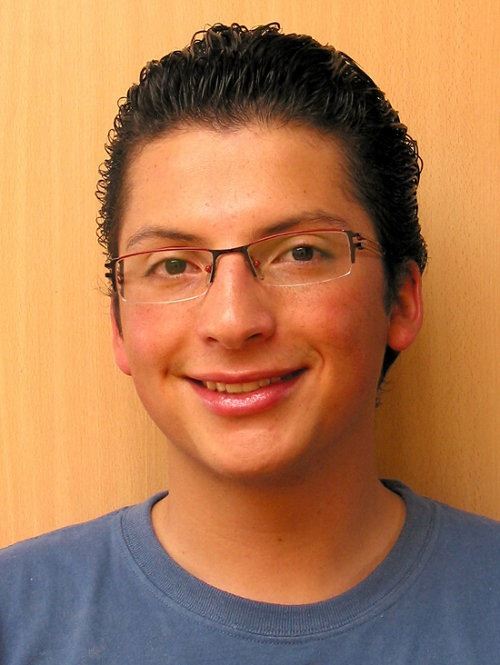
\includegraphics[width=3cm,bb=0 0 500 665]{./foto.jpg}}\\
    Casa \# 2			& {\it mobile:} +(593-9) 643-9206 \\
    Quito, Ecuador		& {\it e-mail:}  najera.oscar@gmail.com\\
				& {\it www:} http://titan-c.github.com
  \end{tabular}\vspace{2cm}


\section{\sc Research Interests}
  Solid State Physics, Statistical Mechanics, scientific programming \&
  computational systems analysis

\section{\sc Education}
  {\bf Escuela Politécnica Nacional}, Quito, Ecuador\\
  \vspace{-.1in}
  \begin{list1}
    \item[] Physics Diploma Student \hfill {\bf August 2006 - present}\\
    \begin{list2}
    \vspace{-.1in}
      \item Thesis Topic:  ``Estimation, by computer simulation, of the exchange
	energy dispersion between polar nano-regions in $Pb_xBi_4Ti_{3+x}O_{12+3x}; x=\{2,3\}$
	relaxor ferroelectrics''
      \item Advisor: Professor Luis Lascano
      \item Expected graduation date: July, 2012
    \end{list2}
  \end{list1}

\section{\sc Honors and Awards}
  Physics Olympiad $1^{st}$ place, Escuela Politécnica Nacional \hfill {\bf 2010}

\section{\sc Academic Experience}
  {\bf Escuela Politécnica Nacional}, Quito, Ecuador

  \vspace{-.3cm}
  {\em Student} \hfill {\bf August 2006 - present}\\
  Includes current research and coursework

  {\em Laboratory and teacher's Assistant} \hfill {\bf August 2011 - present}\\
  Responsible of Experimental Physics laboratory in subjects
  like Newtonian Mechanics, Electromagnetism and Optics.
  Shared responsibility for lectures, homework assignments and grades.

  {\bf International Center for Theoretical Physics}, Trieste, Italy

  \vspace{-.3cm}
  {\em Invited Student} \hfill {\bf Feb 20 - Mar 2, 2012} \\
  Participation and presentation of research work at the {\em ``Advanced School on Scientific
  Software Development''}

\section{\sc Conference Presentations}
  Nájera, O.: ``Phase transitions in random interaction Ising-like models'' {\bf In:} XVI ELAVIO,
  {\em Latin American School in Operations Research}, Feb 2012.

\section{\sc Other Publications}
  Nájera, O.: ``Estimation, by computer simulation, of the exchange energy dispersion between
  polar nano-regions in $Pb_xBi_4Ti_{3+x}O_{12+3x}; x=\{2,3\}$ relaxor ferroelectrics'', Thesis
  Preliminary Examination. Department of Physics - Escuela Politécnica Nacional, April 2012.


\section{\sc Computer Skills}
  \begin{list2}
    \item Languages:  C/C++, Linux shell scripting, Python, Php, Matlab/Octave, \LaTeX
    \item Operating Systems:  Linux(Gentoo)
  \end{list2}

\section{\sc Languages}
  \begin{list2}
    \item Spanish: Native speaker
    \item English: Fluent speaker
    \item German: Fluent speaker
  \end{list2}

\end{resume}
\end{document}
